%It would be interesting to include a section describing the general approach followed to map the different signals/variables in the OPC-UA server to Services in an Arrowhead Local cloud.

%I do not know if this part needs to include details about how the OPC-UA server is configured, or is enough with the information about the services registered in the Service Registry. This last part is what I am most interested, such that an Arrowhead System can use the assembly line to manufacture a product.
The components in the assembly line (Sensors and Actuators) are integrated to Arrowhead cloud as services through the PLC's in-built OPC-UA server.Each of the input (Sensors) and output (Actuators) signals are declared as variables in the OPC-UA server which can be registered in the Arrowhead service registry as read and write services. In Figure  \ref{Figure 1.PNG}, the OPC-UA client contains 20 nodes, out of which 19 nodes refer to the signal values of sensor and actuator, whereas the last node is responsible for triggering the production process in factory.
\begin{figure}[h]
\caption{OPCUA Client}
\label{Figure 1.PNG}
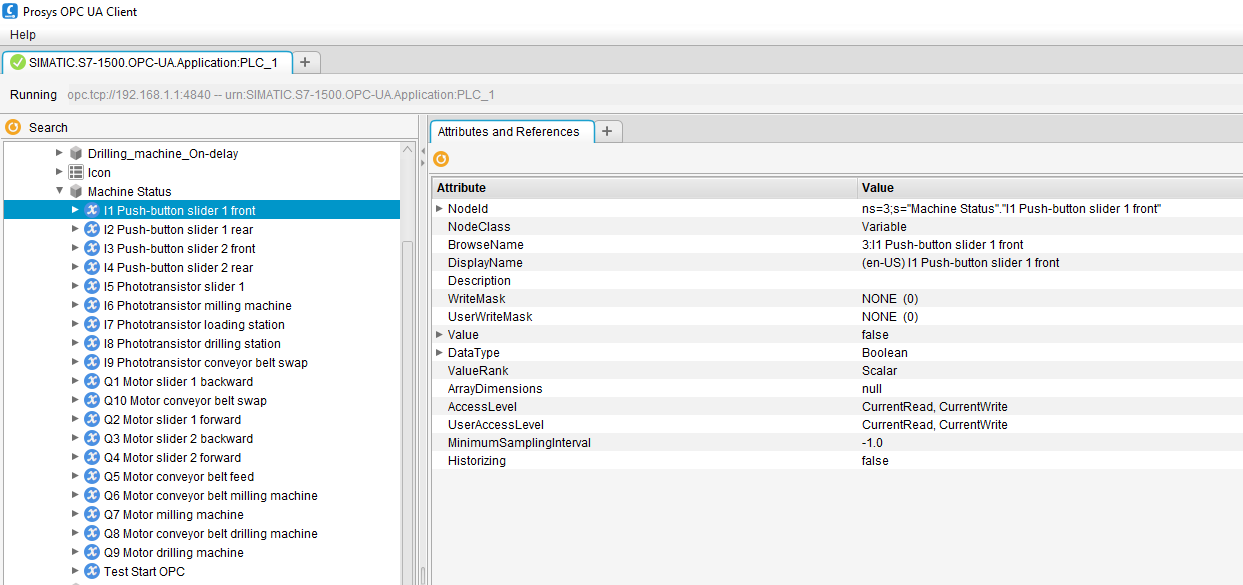
\includegraphics[width=12cm]{Documentation/assemblyLine/sections/Images/OPCUA_Variables.PNG}
\end{figure}

  The sensors and actuators are registering the below services in the Service Registry as illustrated in Figure 2 and 3.
  
  1. Sensors: One GET service, which is responsible for providing the status of the sensor signal (true/false).
  2. Actuators: Two services
        a) One GET service, which is responsible for providing the status of the actuator signal (true/false), 
        b) One POST service, which is responsible for changing the current status of the actuator signal.
  
\begin{figure}[h]
\caption{Arrowhead Services}
\label{Figure 2.PNG}
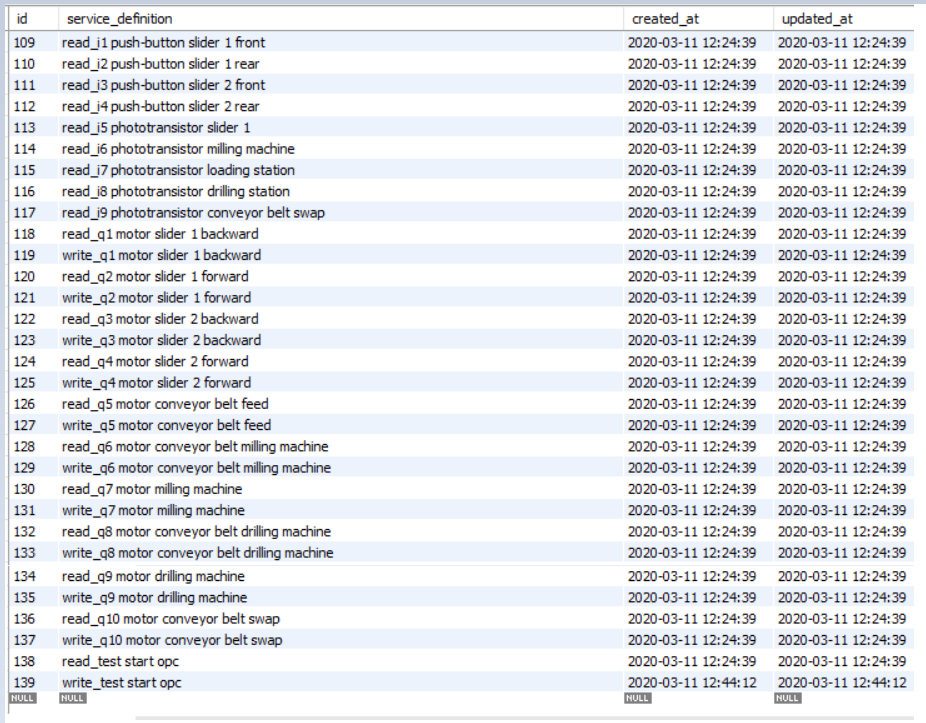
\includegraphics[width=12cm]{Documentation/assemblyLine/sections/Images/Service_Definitions.PNG}
\end{figure}

\begin{figure}[h]
\caption{Service Registry}
\label{Figure 3.PNG}
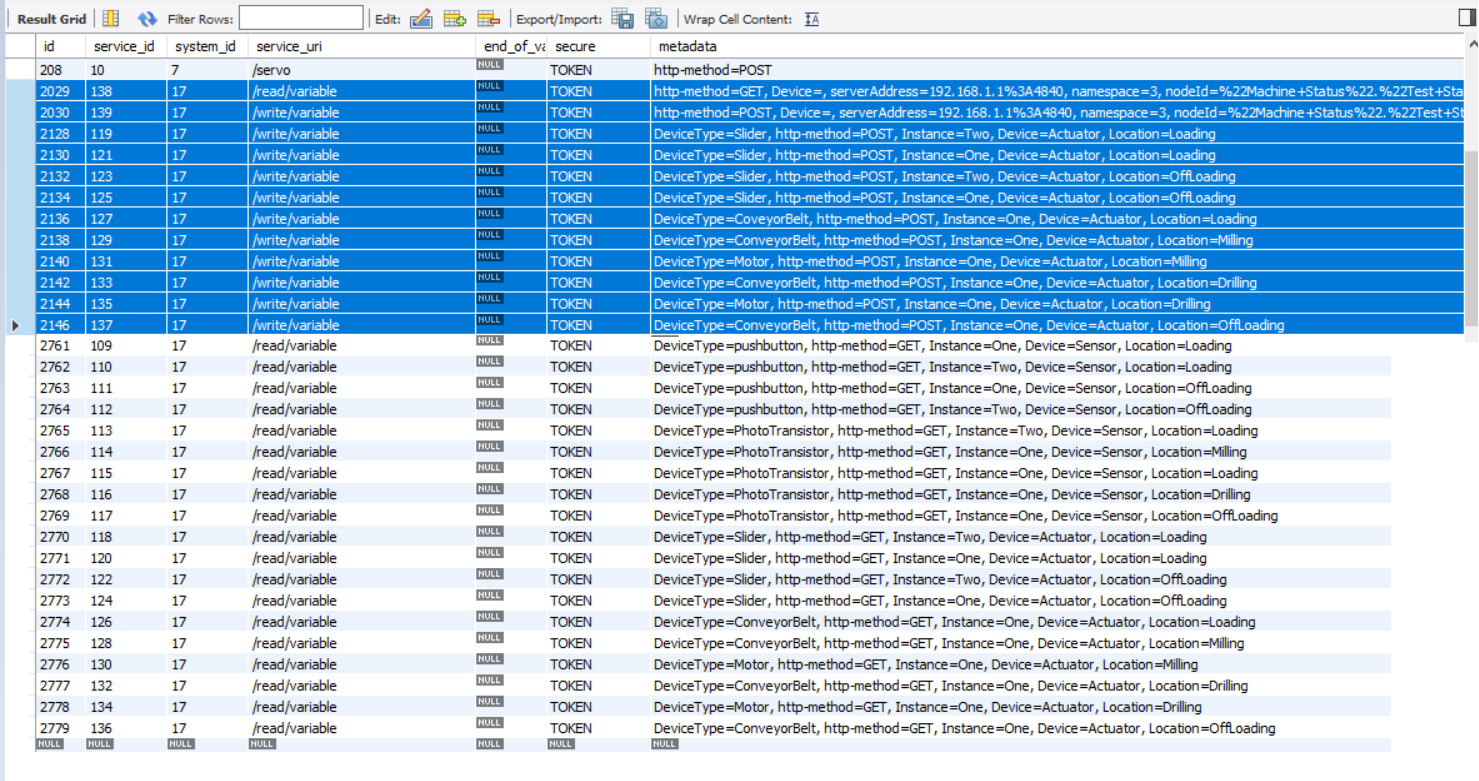
\includegraphics[width=12cm]{Documentation/assemblyLine/sections/Images/ServiceRegistry.png}
\end{figure}
%\end{document}